\documentclass{article}

\usepackage{amsmath,graphicx}

\newcommand{\rr}{\mathbf{r}}

\begin{document}

{\bf Quiz \#4; Tuesday, date: 02/13/2018}

{\bf MATH 53 Multivariable Calculus with Stankova}

{\bf Section \#114; time: 2 -- 3:30 pm}

{\bf GSI name: Kenneth Hung}

{\bf Student name: SOLUTIONS}

\vspace*{0.25in}

\begin{enumerate}
\item Reduce the equation to one of the standard forms, classify the surface, and sketch it.
\[
x^2 - y^2 - z^2 + 2x - 6z - 8 = 0.
\]

{\em Solution.} We start by completing the squares:
\begin{align*}
x^2 - y^2 - z^2 + 2x - 6z - 8 & = 0 \\
(x^2 + 2x) - y^2 - (z^2 + 6z) - 8 & = 0 \\
(x + 1)^2 - y^2 - (z + 3)^2 & = 0.
\end{align*}
Now we can this into a standard form:
\[
(x + 1)^2 = y^2 + (z + 3)^2,
\]
which is the equation of a cone oriented alnog the $x$-axis (i.e.\ elliptic cross sections at $x = k$), centered at $(-1, 0, -3)$. Sketch is as follows:
\begin{center}
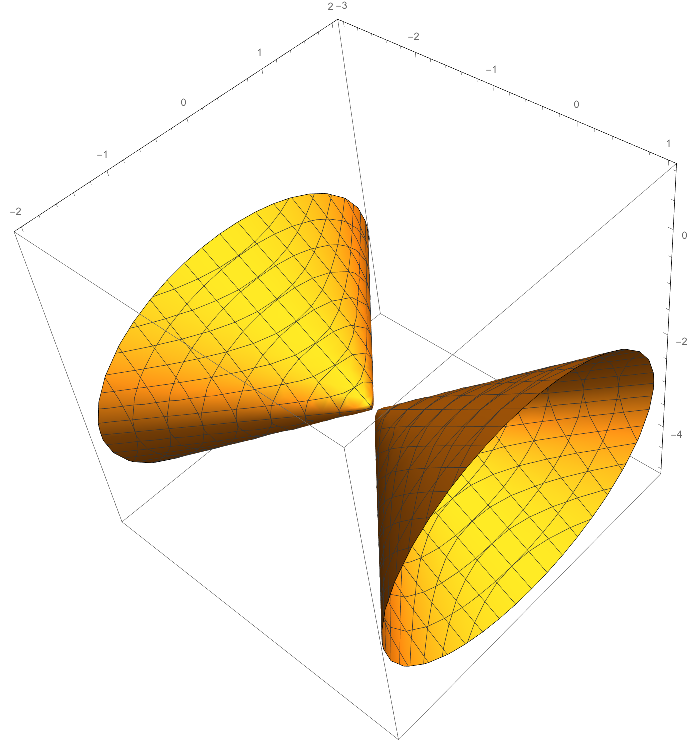
\includegraphics[width=0.7\textwidth]{quiz04dis114solpic}
\end{center}

\item {\em True / False?} Consider a space curve given by the vector equation $\rr(t)$. If all of its projections onto $xy$-plane, $yz$-plane and $xz$-plane are smooth, then the curve itself must be smooth.

{\em Solution.} {\bf True.} Suppose there is such a curve that is not smooth. Then its derivative $\rr'(t)$ must not be defined at some point or is the zero vector. One of its projections onto $xy$-plane, $yz$-plane or $xz$-plane must then have undefined derivative or zero derivative at the same $t$-value, meaning that this projection will not be smooth.

\item {\em True / False?} One of the ways to visualize a space curve is to show it on a surface.

{\em Solution.} {\bf True.} For example to draw the helix, one can draw a cylinder first and show the helix as a curve of the surface of the cylinder for better visualization.
\end{enumerate}

\end{document}